%% Do not edit unless you really know what you are doing.
\documentclass[10pt,english]{article}
\usepackage[T1]{fontenc}
\usepackage[latin1]{inputenc}
\usepackage{fancyhdr}
\pagestyle{fancy}
\setlength\parskip{\medskipamount}
\setlength\parindent{0pt}
\usepackage{graphicx}
\IfFileExists{url.sty}{\usepackage{url}}
                      {\newcommand{\url}{\texttt}}

\makeatletter

%%%%%%%%%%%%%%%%%%%%%%%%%%%%%% LyX specific LaTeX commands.
%% Because html converters don't know tabularnewline
\providecommand{\tabularnewline}{\\}

%%%%%%%%%%%%%%%%%%%%%%%%%%%%%% User specified LaTeX commands.
\usepackage{a4wide}
\usepackage{fancyhdr}

\usepackage{array}
\usepackage{graphicx}
\usepackage{setspace}

\usepackage{auto-pst-pdf}

\lhead{NIKA Prototype: polarisation tests\\}
%\rhead{ \includegraphics[width=2.cm]{logo_tr.eps} }

\usepackage{babel}

\usepackage{babel}
\makeatother
\begin{document}

\title{NIKA Prototype: characterisation of the polarisation capability}


%\author{A. Catalano, A. Ritacco, N. Ponthieu}


%\date{\textbf{Revision/Date:} 01-00 - 2013-09-17}

\maketitle
\bigskip{}

\begin{center}
\includegraphics[width=7cm, , keepaspectratio]{figures/nika_white_bg}\par\end{center}

\vspace{2cm}

\begin{abstract}
This document reports on polarisation lab measurements. The aim of the measurements is to check the consistency of the HWP parameters and the level of instrumental stray polarisation of the NIKA prototype for both 1.25mm and 2.05mm channels. 


We observe that the results are.............



\end{abstract}
%\tableofcontents{}

\section{Document Revision History}

\begin{flushleft}\begin{tabular}{|l|l|l|}
\hline 
Issue&
 Date&
 Changes
 \tabularnewline
\hline
01-00 & 2013-09-17 & First Version
\tabularnewline
\hline
02-00 & 2013-11-03 & Second Version
\tabularnewline
\hline
03-00 & 2013-11-07 & Second Version
\tabularnewline

\hline
\end{tabular}\par\end{flushleft}


\section{Relevant documentation}

This report and additional material can be found on the NIKA svn. ($path$ - \url{home/Processing/Papers_Proposal_Notes/Reports/NIKAPol})
\\
\\
RD 01 Savini et al., Recovering the frequency dependent modulation function of the achromatic half-wave plate for POL-2: the SCUBA-2 polarimeter, APPLIED OPTICS, Vol. 48, No. 11, 10 April 2009.
\\
\\
RD 02 Savini et al., Achromatic half-wave plate for submillimeter instruments in cosmic microwave background astronomy: modeling and simulation, APPLIED OPTICS, Vol. 45, No. 35, 10 December 2006.
\\
\\
RD 03 Pisano et al, Metal-mesh achromatic half-wave plate for use at submillimeter wavelengths, APPLIED OPTICS, Vol. 47, No. 33, 20 November 2008.
\\
\\
RD 04 Hanany, A Millimeter-Wave Achromatic Half Wave Plate, arXiv:physics/0503122v1
\\
\\
RD 05  Fundamentals of Polarized Light, Christian Brosseau, 1998


\section{Introduction}
The NIKA collaboration opened to host a polarised 1.2 mm array in the final NIKA2 instrument. In order to have simultaneous measurement of the three Stokes parameters (I, Q, U) on a same field of the sky through the same optical path in the telescope, we chose to use a rotating half-wave-plate (HWP) at 300K. We chose the continuous rotation strategy to modulate the polarisation. In this mode, a linearly polarised signal is modulated by the combined action of an "ideal" HWP and subsequent analyser at four times the mechanical rotation frequency. It can hence be extracted with a lock-in procedure by isolating the amplitude of the fourth harmonic of the mechanical rotation where the modulation function of the polarised signal is located.
The accuracy of this strategy lies in the calibration of the HWP: the correct amplitude of the various Fourier components relative to different input signals is required in order to decouple unwanted instrumental contaminations from the desired signal.

The performance of the polarisation modulation has to be tested in the NIKA prototype. The NIKA prototype solution for polarisation measurements is the use of a single birefringent sapphire plate. The plate is coated on both sides with a single dielectric substrate in order to minimise surface reflections at what was considered the mean wavelength of the known spectral band (230-240 GHz). This kind of mono-chromatic HWP was preferred to a more sophisticated achromatic HWP in the case of NIKA prototype to minimise and better control all the systematic errors  linked to the plate taking into account the loos of polarisation performances. 

The official NIKA collaboration schedule is to mount the polarisation facilities on the NIKA prototype to observed a first polarised light in the run7 (end of January 2014). 

The purpose of this document is to check the consistency of the HWP parameters and the level of instrumental stray polarisation by testing the whole chain in laboratory with specific tests. 


We performed two sessions of measurements:

\begin{itemize}
\item {\bfseries HWP characterization :} Using Martin-Puplett interferograms we derive the parameters of a real HWP ($\alpha$, $\beta$, inband
Phi, $\rho_{pol}$, ...).
\item  {\bfseries Polarization Systematics of the whole chain:} Total power measurements with rotating HWP in an environment close to the telescope conditions.
\end{itemize}


\section{Test Facility}

Due to a leak of vacuum, the NIKA prototype cryostat was in Neel Institute during the polarisation tests so after fixing the leak it was possible to test the performance of the polarisation system directly in the NIKA prototype instrument.

The HWP is mounted in a mechanical modulator performing the rotation thanks to a stepper motor. All the details about this system can be found in the document  on the NIKA svn. ($path$ - \url{home/Processing/Papers_Proposal_Notes/Reports/doc_MPPSYNC}). As Lumped Elements KIDs used in the NIKA prototype instrument are (at first order) only sensitive to the intensity of the light, we must put a polariser element after the HWP to analyse the modulated polarisation signal. In order to account the optical requirements at the telescope, a lithographic polariser is mounted at a distance of 6cm from the HWP with its substrate plane at 10 degrees with the optical axis to avoid standing waves with the cold optical filters inside the cryostat (see mechanical draw on Fig \ref{fig:setup} right). 

\begin{figure}[t!]
\begin{center}
\includegraphics[width=9cm, , keepaspectratio]{figures/IMG_0955.eps}
\includegraphics[width=5cm, , keepaspectratio]{figures/dessin_final.eps}
\end{center}
\caption{Left: Measurement setup. Right: mechanical draw of the HWP modulator with the analyser support.}
\label{fig:setup}
\end{figure}


The measurement setup is shown in Fig \ref{fig:setup} left. 

\section{Measurements}

In the following subsections we details the laboratory measurements we performed in October 2013. All these measurements have been performed for the 1.25mm channel and the 2.05mm channel.  

\subsection{HWP characterisation}

For this purpose, we performed a spectral measurement of the HWP+NIKA instrument using a polarising Fourier transform spectrometer of the Martin-Puplett kind. The Martin-Puplett produces the difference between the powers of two input polarised beams which are built by two black bodies at different temperatures (ambient eccosorb and warmed eccosorb) modulated by a rotating wire-grid. 
The scan performed has a spectral resolution of about 3.5GHz (about 44 mm of excursion of the roof mirror) with a step of the roof mirror of $250 \mu m $ permitting to cover the two NIKA prototype band pass at 2.05 mm and 1.25mm. 
The Martin-Puplet output signal first feeds into a polyethylene lens that refocus the beam on the KID detectors and then it is selected by a Wire-Grid to have a linear polarisation in a fixed reference position. 

The optical configuration of these measurements is: 

{\bfseries Source} (300K and 100\% polarised from Martin-Puplett )+ {\bfseries HWP} (in a fixed position) + {\bfseries Polaryser} (substrate plane at 10 degrees with the optical axis) + {\bfseries NIKA Cryostat} (Cold Optics and KIDs)

We measured several spectra at different angles of the HWP with respect to the optical axis in order to study the attenuation of the spectrum versus frequencies produced by the HWP convolved with NIKA prototype bandpass. In principle by using a model accounting the real HWP mueller matrix (see equation on annex 1) we can derive the the parameters of the HWP. 

\begin{table*} 
  \begin{center}
  \scalebox{1}{%
    \begin{tabular}{cccc}
      \hline
      & Diameter [mm] &  Thickness [mm] & Working Freq.[GHz]  \\
      \hline  \hline	
       & 100 & 1.97 & 230 \\
    \hline  \hline
    \end{tabular}
 }
  \end{center}
  \caption{Half Wave Plate characteristics} \label{tab1}
\end{table*}


\subsection{Instrumental stray polarisation characterisation}

In order to check all the systematics we should face at the telescope, we performed total power measurements with rotating HWP at a typical mechanical rotation frequency (1.9Hz) using the sky simulator (about 50K) as a not polarised source. In this case, as we do not use a modulated source to lock-in we expect to observe a certain amount of ambient polarisation of the room. 

The rotation speed was chosen in order to produce 12 measurements per mechanical tour synchronised to the sampling frequency. This allowed us to recover 3 samples per optical tour which is still enough to reconstruct $S_o$ $S_1$ and $S_2$ stokes parameters. 

The measurements have been performed in three different configurations:

{\bfseries- Telescope conditions : } the source feeds through the rotating HWP and the analyser. In this case we repeated the same measurement changing the angle of the analyser by 30 degrees.

{\bfseries - Polarisation And Flux systematics 1:} the source feeds only through the rotating HWP.

{\bfseries - Polarisation And Flux systematics 2:} the source feeds only through the rotating modulator without the HWP.


\subsection{Activities list and date performed}
The detailed list of the performed measurements and the data references are presented in Annex 2.
 
\section{Data reduction}

\subsection{HWP parameters}

We do not have enough information to characterise each element individually. For our goals, it is however reasonable to assume that the polarisers used in the measurements have a negligible cross-polarization. We assume hereafter to use ideal polarisers so we will focus only on the characterisation of the HWP parameters.
\\
\\
\\
First we measured a spectrum with the HWP aligned to its speed axis w.r.t. the two polarysers (0 deg in the log book). This corresponds to the maximum signal  in which we expect to have no distortion of the NIKA bandpass. We used this measured spectrum as a reference spectrum to a analytical model based on the formalism presented in Annex 1. By rotating the HWP angle, we expect to observe a different attenuation for each wavelength due to the linear relation between the phase shift and the wavelength (see Annex 1). This effect is expected to be quite strong because the HWP is not achromatic. 
\\
\\
\\
We measured several spectrum ad different HWP angles in order to compare the measured spectra with the analytical model. Since the constant 300K background on pixels can change a lot when we title the HWP it is very important to recenter the tone for each detector for each position in order to be able to compare properly the measured spectra.
In Fig.\ref{fig:respar}  we present this analysis. In these conditions we can fit the principal parameters of the model of a real HWP. These results are presented on table\ref{tab2}.
\\
\\
\\
\\
When the $\alpha$, $\beta$ and $\phi$ parameters are determined, we can derive the polarisation efficiency in-band. 
From Eq.\ref{eq:real_hwp} we can define the HWP polarisation efficiency as $\rho_{pol} = (1-2\gamma)/2$ where $\gamma = \frac{\alpha \beta \cos(\phi)}{\alpha^2 + \beta^2}$. By multiplying $\rho_{pol}$ to the intensity spectral bandpass we obtain the $Q-U$ spectra shown in Fig.\ref{fig:IQband}



\begin{figure}[t!]
\begin{center}
\includegraphics[width=6.5cm , keepaspectratio]{figures/Spectrum_HWP_1mm.ps}
\includegraphics[width=6.5cm , keepaspectratio]{figures/Attenuation_HWP_1mm.ps} \\
\includegraphics[width=6.5cm , keepaspectratio]{figures/Spectrum_HWP_2mm.ps}
\includegraphics[width=6.5cm , keepaspectratio]{figures/Attenuation_HWP_2mm.ps} \\
\end{center}
\caption{Results of the HWP parameter characterisation.}
\label{fig:respar}
\end{figure}

\begin{figure}[t!]
\begin{center}
\includegraphics[width=9cm , keepaspectratio]{figures/final_spectrum.ps}
\end{center}
\caption{Intensity spectrum (red) and Q-U spectrum (blue) for the two NIKA prototype channels.}
\label{fig:IQband}
\end{figure}


\subsection{Instrumental stray polarisation}
In this section we will focus on the study of the polarisation signal in the configuration telescope, with the rotating HWP in the configuration as introduced.
In order to point out the differences between the 1.25mm matrix and the 2 mm matrix we show the Fig \ref{fig:mod}.
\\
\begin{figure}[b!]
\begin{center}
\includegraphics[width=4.5cm , keepaspectratio]{figures/Modulation_SS_1mm.ps} 
\includegraphics[width=4.5cm , keepaspectratio]{figures/Modulation_SS_HWP_1mm.ps} 
\includegraphics[width=4.5cm , keepaspectratio]{figures/Modulation_SS_HWP_WG_1mm.ps} \\
\includegraphics[width=4.5cm , keepaspectratio]{figures/Modulation_SS_2mm.ps} 
\includegraphics[width=4.5cm , keepaspectratio]{figures/Modulation_SS+HWP_2mm.ps} 
\includegraphics[width=4.5cm , keepaspectratio]{figures/Modulation_SS+HWP+WG_2mm.ps} 
\end{center}
\caption{Typical time lines observed for 1.25mm channel (3 top plots) and for 2mm channel (3 bottom plots): left plot is the signal recovered without HWP and without the polariser. Only the mechanical modulator is in rotation. Central plot is the signal with only the rotating HWP. Right plot is the signal with rotating HWP and the polariser in a fixed position.}
\label{fig:mod}
\end{figure}
\\
\\
The Fig \ref{fig:pow} shows the intensity of the polarisation signal at 8 Hz corresponding to four time the mechanical rotation frequency of the HWP. Also in this case we show the power spectra for the 1.25mm channel and for the 2mm channel.

\begin{figure}[t!]
\begin{center}

\includegraphics[width=7cm , keepaspectratio]{figures/1mm_Power_spectre_tot.ps}
\includegraphics[width=7cm , keepaspectratio]{figures/2mm_Power_spectre_tot.ps} 
\end{center}
\caption{Power Spectrum for 1.25mm channel (left) and for 2mm channel (right)}
\label{fig:pow}
\end{figure}

It's interesting to compare the results obtained by the previous characterization with the data obtained by the rotating HWP configuration. 
\\
The idea is to verify  the consistency of the model used to obtain the instrumental parameters.
The initial purpose was to compare simply the signal measured in the laboratory during the preliminary session of measures with the model obtained from the measurements with MPI but there was a problem with the sampling, due to an incorrect setting of the acquisition parameters and therefore it was impossible reconstructing the real signal observed. The signal  measured was inconsistent with the signal expected.
So, once we understand the problem and still wanting to check the consistency of the model and therefore the instrumental parameters calculated, we have taken in consideration the data measured at the telescope without the source observed, with the cabin as ambient. Thanks to these data we are able to reconstruct the real polarized signal.
The model reproduces the signal with the harmonics to $2\omega$ and $4\omega$ instead we have the signal at all frequencies.
The goal is fit the signal in order to find the amplitudes of the signal at several frequencies and then to separate the components to $2\omega$ and $4\omega$ and reconstruct the signal with just these components.
\\
\\
\\ 
\begin{figure}[h!]
\begin{center}
\includegraphics[width=7cm , keepaspectratio]{figures/Petit_timeline.ps}
\includegraphics[width=7cm , keepaspectratio]{figures/2Petit_timeline.ps}
\end{center}
\caption{Signal observed for the 1.25mm channel (left) and 2mm channel (right) on a little timeline with the fit in blue }
\label{fig:ptl}
\end{figure}
\\
\\
\\
In the Fig \ref{fig:ptl} we show the accuracy of the fit. So, we have obtained the amplitudes. It was made the same procedure to calculate the amplitudes of the signal simulated with the model of an ideal HWP in order to establish the content in more polarization, because the model includes a signal cleaned without to consider the eventually components added to polarization created by external ambient.
The same procedure is made for the 2mm channel because if there is polarization added for the 1.25 mm channel there is also for the 2mm channel. 
\\
\\
If we consider the equation:
\begin{equation}\label{emme}
m = (A+B) \cos{2(\omega+\phi)} + (B+\frac{1-2\gamma}{2})\cos{4 (\omega+\phi)}
\end{equation}
where $\phi$ is the phase shift induced by the birefringence and $\gamma$ = $T_1T_2 \cos(\phi)/(T_1^2T_2^2)$
and B =$ (T_1^2-T_2^2)/(T_1^2+T_2^2)$. Let's call $T_1$ and $T_2$ the transmission parameters of the HWP along its fast and slow axis.
B can be interpreted as the differential transmission between the fast and slow axis, $\phi$ monitors the phase shift induced by the HWP thickness.
The Eq \ref{emme}  represents the signal measured with just the components of interest and the terms between parentheses represent the amplitudes for the components to 2 $\omega$ and 4 $\omega$. 
So, by the their ratio for the amplitudes of the two channels we find in the case of the 2mm channel a ratio of 1.4 and for the model 3.4. Instead for the 1.25mm channel we find a ratio of 19 and for the model of 9. In both cases the difference between the ratio of the real signal amplitudes and that simulated by the model is about two.
Therefore if I define $\rho$ =$\frac{B}{A}$  it's possible to demonstrate from the Eq  \ref{emme} to be equals the ratio of the amplitudes of the model and of the data respectly.
Since $\rho$ results comparable in the two cases it's possible to deduce that there's in more than a fraction of polarization that the model doesn't consider.
\section{Conclusion}

\newpage
\section*{Annex 1 : Elements of Jones and Stokes formalism.}

In this section we present some element of the formalism that we permit to built a model used to fit the HWP parameters.

\subsection*{Polarisation of light}
Light is described as a phenomenon due to the electromagnetic field oscillations throughout the space. If we consider a Cartesian coordinate system $(x,y,z)$, where $z$ is for convenience the propagation axis, the oscillation of the electromagnetic field has to satisfy the $D'Alembert$ equation: 

\begin{equation}\label{alembert}
\nabla^2 E_i (r,t) = \frac{1}{c^2} \frac{\partial^2 E_i(r,t)}{\partial t}
\end{equation}   

Solving the Eq \ref{alembert} considering the isofrequency solutions we find:

\begin{eqnarray}\label{elfield}
E_x(z,t) & = & E_{0x} \cos{ (\tau + \delta_x )} \nonumber \\
E_y(z,t) & = & E_{0y} \sin{(\tau + \delta_y )}
\end{eqnarray}

We can derive the locus described by the resultant vector as:

\begin{equation}\label{ellipse}
\frac{E_x^2}{E_{0x}^2}+\frac{E_{y}^2}{E_{0y}^2}-2\frac{E_{x}}{E_{0x}}\frac{E_{y}}{E_{0y}} \cos{\delta} = \sin{\delta}
\end{equation}  

where $\delta = \delta_x - \delta_y$. The Eq \ref{ellipse} is defined as $polarisation$ $ellipse$ and it represents in a general form all the polarisation status of light. 
Depending on particular values of $\delta$ or/and $E_{0xy}$ polarisation ellipse falls into particular forms.

\begin{itemize}
\item {\bfseries Linear Polarisation} (in the x or y direction) : if $E_{0x} = 0$ or $E_{0y}=0$ 
\item {\bfseries Linear Polarisation} (45 degrees) : if $\delta = 0$ or $\delta=\pi$ and $E_{0x} = E_{0y} = E_{0} $
\item {\bfseries Cicular Polarisation} (clockwise or anticlockwise) : if $\delta = \pi/2$ or $\delta=3/2 \pi$ and $E_{0x} = E_{0y} = E_{0} $ 
\end{itemize}

\subsection*{Jones Calculus}
It is possible to describe polarised light by a $Jones$ vector, and linear optical elements by $Jones$ $matrices$. When light crosses an optical element the resulting polarisation of the emerging light is found by taking the product of the Jones matrix of the optical element and the Jones vector of the incident light as follow:

\begin{eqnarray}
\left(\begin{array}{c}
E^{'}_x(t) \\
E^{'}_y(t) \end{array}\right) & = & \left(\begin{array}{cr}
J_{00} & J_{01} \nonumber \\
J_{11} & J_{12}
\end{array}\right)
\left(\begin{array}{c}
E_x(t) \\
E_y(t) \end{array}\right) \label{eq:jones}\\
\end{eqnarray}

For many applications, it is interesting to deal with rotated active optical elements. Indeed, the rotation by a angle $\theta$ of an element induces a variation of the polarisation status.

If we change the Cartesian coordinates system we obtain:
\begin{eqnarray}\label{rotation}
E^{'}_{x} & = & E_{x} \cos{ ( \theta )} +  E_{y} \sin{ ( \theta )} \nonumber \\
E^{'}_{y} & = &  - E_{x} \sin{ ( \theta )} +  E_{y} \cos{ ( \theta )}
\end{eqnarray}
  
We can derive the $Jones$ matrix of a rotated system as:
\begin{eqnarray}
M(\theta) & = & \left(\begin{array}{cr}
\cos{ ( \theta )} & \sin{ ( \theta )} \nonumber \\
- \sin{ ( \theta )} & \cos{ ( \theta )}
\end{array}\right)
 \label{eq:jonesrot}\\
\end{eqnarray}

  
In order to efficiently estimate the outgoing polarisation, it is necessary to trasform the coordinate system forward to the initial reference. We obtain:

\begin{equation}
S^{'} = M^T(\theta) \cdot M_{el} \cdot M(\theta)
\end{equation} 

Where $M_{el}$ is the generic optical element. 


For the purposes of this report, we derive the jones matrix of a (ideal and real) generic polariser and an (ideal and real) generic half wave plate:  

\begin{itemize}
\item {\bfseries Ideal Polariser}
 
An linear polariser consists of a regular array of fine parallel lithographic or metallic wires, placed in a plane perpendicular to the incident beam. In a ideal generalisation the electromagnetic waves which have a component of their electric fields aligned parallel to the wires the wave is fully reflected backwards along the incident beam. On the other hand, the perpendicular component is fully transmitted.

If we consider a specific case in which the transmission on the x-axis ($\alpha=1$) is 1 and 0 on y-axis ($\beta =0$) we obtain:

\begin{eqnarray}
\left(\begin{array}{cr}
c^2 & c\cdot s \nonumber \\
c\cdot s& s^2
\end{array}\right)
\label{eq:ideal:pol}
\end{eqnarray}

where $c=\cos{\theta}$ and $s=\sin{\theta}$
 
\item {\bfseries Real Polariser} 
In this case we generalise the ideal case by supposing that $\alpha$ and $\beta$ are both different from 0. We obtain:

\begin{eqnarray}
\left(\begin{array}{cr}
\alpha \cdot c^2 + \beta \cdot s^2 & (\alpha-\beta)\cdot c \cdot s \nonumber \\
 (\alpha-\beta)\cdot c \cdot s & \alpha \cdot c^2 + \beta \cdot s^2
\end{array}\right)
\label{eq:real:pol}
\end{eqnarray}

\item {\bfseries Ideal Half Wave Plate} 

For a birefringent material, two orthogonal directions define the ``ordinary
axis'' and the ``extraordinary axis'' that have a different optical index $n_o$
and $n_e$. An incident electric field has components along both directions, and
while passing through the plate, they are shifted differently, which induces a
rotation of polarisation. This shift in the case of a single sapphire plate can be written as:

\begin{equation}
\Delta \phi = 2\pi (n_e-n_o) d / \lambda\;.
\label{eq:shift}
\end{equation}

where $d$ is the optical path inside the element and $\lambda$ is the wavelenght.
Eq.~(\ref{eq:shift}) shows that the phase shift induced by the plate depends on
both the optical index and the thickness is we always work at normal incidence. 


Let's assume that $x$ is the ordinary axis and $y$ the extraordinary axis. In an ideal HWP we assume that the transmission along the two axis ($\alpha$ and $\beta$) are equal to 1. In addition we assume that the HWP works at one wavelength in which we have a phase-shift  of $\Delta \phi = \pi$. We obtain the Jones matrix: 

\begin{eqnarray}
\left(\begin{array}{cr}
c_2 & s_2 \nonumber \\
s_2 & -c_2
\end{array}\right)
\label{eq:ideal:hwp}
\end{eqnarray}

where $c_k=\cos{k \theta}$ and $s_k=\sin{k \theta}$.

\item {\bfseries Real Half Wave Plate} 

In this case we generalise the Eq.\ref{eq:ideal:hap} by supposing that $\alpha$ and $\beta$ are both different from 1 and as in a real instrument we do not work with one wavelength, we keep the phase-shift as a free parameter. We obtain: 

\begin{eqnarray}
\left(\begin{array}{cr}

\end{array}\right)
\label{eq:real:hwp}
\end{eqnarray}

\end{itemize}

\subsection*{Stokes formalism}

Stoke formalism represents the more common description of incoherent or partially polarised radiation in terms of its total intensity, the degree of polarisation, and the shape parameters of the polarisation ellipse. Indeed the stoke formalism accounts a measurable representation of the electromagnetic field by using time averages of $E_x(t)$ and $E_y(t)$.

Starting from Eq.\ref{ellipse} we can obtain the 4 Stokes parameters by averaging over a period of electromagnetic oscillation:

\begin{eqnarray}\label{stokes}
S_o & = & E_{xo}^2 + E_{yo}^2  \nonumber \\
S_1 & = & E_{xo}^2 - E_{yo}^2  \nonumber \\
S_2 & = & 2E_{xo}E_{yo} \cos{\delta}   \nonumber \\
S_3 & = & 2E_{xo}E_{yo} \sin{\delta}
\end{eqnarray}

Using this notation we can write the Eq \ref{ellipse} as:

\begin{eqnarray}\label{stokes}
S_o^2 & = & S_1^2 + S_2^2 +S_3^2 
 \label{eq:stoke_p}
\end{eqnarray}

\begin{itemize}

\item $S_o$ represents the total intensity.
\item $S_1$ is the amount of horizontal and vertical linear polarisation. 
\item $S_2$ represents the linear polarisation at 45 degrees. 
\item $S_3$ represents the clockwise and anti clockwise circular polarisation.

\end{itemize}

For the NIKA polarisations astrophysical aims we are interested only on linear polarisation, for this reason from hereafter we account only the first 3 stokes parameters $S_o$, $S_1$ and $S_2$.
In general it results that for light partially polarised: 

\begin{eqnarray}\label{stokes}
S_o^2 & \geq & S_1^2 + S_2^2 +S_3^2 
 \label{eq:stoke_p}
\end{eqnarray}

where the equal corresponds to the total polarised light case. 

In order to manipulate the Stokes vectors to interact with optical elements, we can use the Mueller matrix. We give here the basic relations between Jones and Mueller matrix:

\begin{eqnarray}
M_{kl} & = &  \frac{1}{2}\left(\begin{array}{rrr}
|J_{00}|^2 + |J_{01}|^2 + |J_{10}|^2 + |J_{11}|^2 &
|J_{00}|^2 - |J_{01}|^2 + |J_{10}|^2 - |J_{11}|^2 &
2Re(J_{00}J_{01} + J_{10}J_{11}) \nonumber \\

|J_{00}|^2 + |J_{01}|^2 - |J_{10}|^2 - |J_{11}|^2 &
|J_{00}|^2 - |J_{01}|^2 - |J_{10}|^2 + |J_{11}|^2 &
2Re(J_{00}J_{01} - J_{10}J_{11}) \nonumber \\

2Re( J_{00}J_{10} + J_{01}J_{11}) &
2Re( J_{00}J_{10} - J_{01}J_{11}) &
2Re( J_{00}J_{11} + J_{01}J_{10})\end{array}\right) \nonumber \label{eq:jones2mueller_2}
\end{eqnarray}

In the following we derive the Mueller matrixes for a real polariser and a real HWP only in case of linear polarisation.

\begin{itemize}

\item {\bfseries Real Polariser} 

\begin{eqnarray}
M_{POL} &=& \frac{1}{2}\left(\begin{array}{lll}
\alpha^2+\beta^2              & (\alpha^2-\beta^2) c_2 & (\alpha^2-\beta^2) s_2 \nonumber \\
(\alpha^2-\beta^2) c_2 & (\alpha^2-\beta^2) c_2^2+ 2\alpha \beta\cdot s_2^2 & (\alpha^2-\beta^2) c_2 s_2  \nonumber \\
(\alpha^2-\beta^2) s_2 & (\alpha^2-\beta^2) c_2 s_2 & (\alpha^2-\beta^2) s_2^2+ 2\alpha \beta
\end{array}\right)\label{eq:real_pol}
\end{eqnarray}

\item {\bfseries Real Half Wave Plate} 

\begin{eqnarray}
M_{HWP} &=& \frac{1}{2}\left(\begin{array}{lll}
\alpha^2+\beta^2              & (\alpha^2-\beta^2) c_2 & (\alpha^2-\beta^2) s_2   \\
(\alpha^2-\beta^2)\cdot c_2 & (\alpha^2+\beta^2) c_2^2+ 2\alpha \beta s_2^2 \cos{\phi} & (\alpha^2+\beta^2-2\alpha \beta \cos{\phi})c_2 s_2   \\
(\alpha^2-\beta^2) s_2 &  (\alpha^2+\beta^2-2\alpha \beta \cos{\phi})c_2 s_2 & (\alpha^2+\beta^2) s_2^2+ 2\alpha \beta c_2^2 \cos{\phi}
\end{array}\right)\label{eq:real_hwp}
\end{eqnarray}

\end{itemize}


\section*{Annex 2 :  LOGBOOK: NIKA Polarisation Measurements}


{\bfseries15/10/2013 Interferometer Session 1MM ARRAY }

\begin{itemize}

\item WG // no HWP 1mm array:

interfero nb mess / per = 5 dur�e acc. = 1 mini = -22 max= 22   micros par sec (step) 80 (phase lock-in 1)

file (bambini and archeops 5) 2013 10 15 10h06m  (file fits tt\_2013\_10\_15\_10h15m21\_ref\_noHWP\_1mm and tt\_2013\_10\_15\_14h30m35\_noHWP\_1mm\_1.fits)

\item WG // no HWP 2mm array:

interfero nb mess / per = 5 dur�e acc. = 1 mini = -22 max= 22  micros par sec (step) = 80 (phase lock-in 0)

file (bambini and archeops 5) 2013 10 15 10h45m  (file fits tt\_2013\_10\_15\_10h54m37\_ref\_noHWP\_2mm.fits)

\item WG //  HWP  speed/crystal axis 1mm array:

interfero nb mess / per = 5 dur�e acc. = 1 mini = -22 max= 22  micros par sec (step) = 80 (phase lock-in 1)

file (bambini and archeops 5) 2013 10  problems on reading raw data only fits available (file fits tt\_2013\_10\_15\_12h59m56\_HWP0\_1mm.fits tt\_2013\_10\_15\_15h22m15\_HWP0\_1mm.fits)

\item WG //  HWP  speed/crystal axis + about 22.5�  1mm array:

interfero nb mess / per = 5 dur�e acc. = 1 mini = -22 max= 22  micros par sec (step) = 80 (phase lock-in 1)

file (bambini and archeops 5) 2013 10  problems on reading raw data only fits available (file fits tt\_2013\_10\_15\_15h50m48\_HWP22d5p\_1mm)

\item WG //  HWP  speed/crystal axis + about 45�  1mm array:

interfero nb mess / per = 5 dur�e acc. = 1 mini = -22 max= 22  micros par sec (step) = 80 (phase lock-in 1)

file (bambini and archeops 5) 2013 10  problems on reading raw data only fits available (file fits tt\_2013\_10\_15\_16h54m47\_HWP45\_1mm)

\item WG //  HWP  speed/crystal axis + about 90�  1mm array:

interfero nb mess / per = 5 dur�e acc. = 1 mini = -22 max= 22  micros par sec (step) = 80 (phase lock-in 1)

file (bambini and archeops 5) 2013 10  problems on reading raw data only fits available (file fits tt\_2013\_10\_15\_16h54m47\_HWP90\_1mm)

\item WG //  HWP  speed/crystal axis + about 90�+epsilon  1mm array:

interfero nb mess / per = 5 dur�e acc. = 1 mini = -22 max= 22  micros par sec (step) = 80 (phase lock-in 1)

file (bambini and archeops 5) 2013 10  problems on reading raw data only fits available (file fits tt\_2013\_10\_15\_17h15m35\_HWP90peps\_1mm)

\item WG //  HWP  speed/crystal axis + about 90�-epsilon  1mm array:

interfero nb mess / per = 5 dur�e acc. = 1 mini = -22 max= 22  micros par sec (step) = 80 (phase lock-in 1)

file (bambini and archeops 5) 2013 10  problems on reading raw data only fits available (file fits tt\_2013\_10\_15\_17h29m10\_HWP90meps\_1mm)

\item WG //  HWP  speed/crystal axis + about 0�+epsilon  1mm array:

interfero nb mess / per = 5 dur�e acc. = 1 mini = -22 max= 22  micros par sec (step) = 80 (phase lock-in 1)

file (bambini and archeops 5) 2013 10  problems on reading raw data only fits available (file fits tt\_2013\_10\_15\_17h52m39\_HWP0peps\_1mm)

\item WG //  HWP  speed/crystal axis + about 0�-epsilon  1mm array:

interfero nb mess / per = 5 dur�e acc. = 1 mini = -22 max= 22  micros par sec (step) = 80 (phase lock-in 1)

file (bambini and archeops 5) 2013 10  problems on reading raw data only fits available (file fits tt\_2013\_10\_15\_18h05m04\_HWP0meps\_1mm)

\item WG //  HWP  speed/crystal axis + about 30�  1mm array  (16/10/2013):

interfero nb mess / per = 5 dur�e acc. = 1 mini = -22 max= 22  micros par sec (step) = 80 (phase lock-in 1)

file (bambini and archeops 5) 2013 10  problems on reading raw data only fits available (file fits tt\_2013\_10\_16\_07h23m47\_HWP30\_1mm)
\end{itemize}

{\bfseries16/10/2013 Rotating HWP Session 1MM ARRAY }

\begin{itemize}
\item Ref meas. WG 0 HWP. Rotating Modulator at 1.9HZ. (!):

Modulation control: vitesse2 = 3600 (the sped for 1meas/tour : 43200 optical to ration (4xmechanical)) 3600 corresponds to 3 meas per optical tour -- pas par tour 6399
file (bambini and archeops 5) 2013 10 16 14h40m08

\item  Ref meas. WG 30  HWP. Rotating Modulator at 1.9HZ. (!):

Modulation control: vitesse2 = 3600 (the sped for 1meas/tour : 43200 optical to ration (4xmechanical)) 3600 corresponds to 3 meas per optical tour -- pas par tour 6399
file (bambini and archeops 5) 2013 10 16 14h49m04

\item Ref meas. WG 60 HWP. Rotating Modulator at 1.9HZ. (!):

Modulation control: vitesse2 = 3600 (the sped for 1meas/tour : 43200 optical to ration (4xmechanical)) 3600 corresponds to 3 meas per optical tour -- pas par tour 6399
file (bambini and archeops 5) 2013 10 16 15h06m56

\item  Ref meas. WG 90 HWP. Rotating Modulator at 1.9HZ. (!):

Modulation control: vitesse2 = 3600 (the sped for 1meas/tour : 43200 optical to ration (4xmechanical)) 3600 corresponds to 3 meas per optical tour -- pas par tour 6399
file (bambini and archeops 5) 2013 10 16 15h13m17

\item  Ref meas. WG 150 HWP. Rotating Modulator at 1.9HZ.:

Modulation control: vitesse2 = 3600 (the sped for 1meas/tour : 43200 optical to ration (4xmechanical)) 3600 corresponds to 3 meas per optical tour -- pas par tour 6399
file (bambini and archeops 5) 2013 10 16 15h26m57

\item  Ref meas. WG 180 HWP. Rotating Modulator at 1.9HZ. (!):

Modulation control: vitesse2 = 3600 (the sped for 1meas/tour : 43200 optical to ration (4xmechanical)) 3600 corresponds to 3 meas per optical tour -- pas par tour 6399
file (bambini and archeops 5) 2013 10 16 15h35m24

\item  Ref meas. WG 210 HWP. Rotating Modulator at 1.9HZ. (!):

Modulation control: vitesse2 = 3600 (the sped for 1meas/tour : 43200 optical to ration (4xmechanical)) 3600 corresponds to 3 meas per optical tour -- pas par tour 6399
file (bambini and archeops 5) 2013 10 16 15h43m54

\item  Ref meas. WG 270 HWP. Rotating Modulator at 1.9HZ. (!):

Modulation control: vitesse2 = 3600 (the sped for 1meas/tour : 43200 optical to ration (4xmechanical)) 3600 corresponds to 3 meas per optical tour -- pas par tour 6399
file (bambini and archeops 5) 2013 10 16 15h59m05

\item  Ref meas. WG 270 HWP. Rotating Modulator at 1.9HZ. (!):

Modulation control: vitesse2 = 3600 (the sped for 1meas/tour : 43200 optical to ration (4xmechanical)) 3600 corresponds to 3 meas per optical tour -- pas par tour 6399
file (bambini and archeops 5) 2013 10 16 15h59m05

\item  Ref meas. WG 300 HWP. Rotating Modulator at 1.9HZ. (!):

Modulation control: vitesse2 = 3600 (the sped for 1meas/tour : 43200 optical to ration (4xmechanical)) 3600 corresponds to 3 meas per optical tour -- pas par tour 6399
file (bambini and archeops 5) 2013 10 16 16h08m48

\item  Ref meas. WG 330 HWP. Rotating Modulator at 1.9HZ. (!):

Modulation control: vitesse2 = 3600 (the sped for 1meas/tour : 43200 optical to ration (4xmechanical)) 3600 corresponds to 3 meas per optical tour -- pas par tour 6399
file (bambini and archeops 5) 2013 10 16 16h15m01

\item  Ref meas. WG 120 HWP. Rotating Modulator at 1.9HZ. (!):

Modulation control: vitesse2 = 3600 (the sped for 1meas/tour : 43200 optical to ration (4xmechanical)) 3600 corresponds to 3 meas per optical tour -- pas par tour 6399
file (bambini and archeops 5) 2013 10 16 16h21m08

\item  Ref meas. no WG HWP. Rotating Modulator at 1.9HZ. (!):

Modulation control: vitesse2 = 3600 (the sped for 1meas/tour : 43200 optical to ration (4xmechanical)) 3600 corresponds to 3 meas per optical tour -- pas par tour 6399
file (bambini and archeops 5) 2013 10 16 16h28m25

\item  Ref meas. no WG no HWP. Rotating Modulator at 1.9HZ. without TOP(!):

Modulation control: vitesse2 = 3600 (the sped for 1meas/tour : 43200 optical to ration (4xmechanical)) 3600 corresponds to 3 meas per optical tour -- pas par tour 6399
file (bambini and archeops 5) 2013 10 16 16h46m42

\item  Ref meas. no WG no HWP. Rotating Modulator at 1.9HZ. with TOP (!):

Modulation control: vitesse2 = 3600 (the sped for 1meas/tour : 43200 optical to ration (4xmechanical)) 3600 corresponds to 3 meas per optical tour -- pas par tour 6399
file (bambini and archeops 5) 2013 10 16 16h54m43
\end{itemize}

{\bfseries17/10/2013 Rotating HWP Session 2MM ARRAY }

\begin{itemize}
\item  Ref meas. no WG no HWP. Rotating Modulator at 1.9HZ. with TOP (!):

Modulation control: vitesse2 = 3600 (the sped for 1meas/tour : 43200 optical to ration (4xmechanical)) 3600 corresponds to 3 meas per optical tour -- pas par tour 6399
file (bambini and archeops 5) 2013 10 17 07h45m22

\item  Ref meas. no WG no HWP. Rotating Modulator at 1.9HZ. without TOP (!):

Modulation control: vitesse2 = 3600 (the sped for 1meas/tour : 43200 optical to ration (4xmechanical)) 3600 corresponds to 3 meas per optical tour -- pas par tour 6399
file (bambini and archeops 5) 2013 10 17 07h58m47

\item  Ref meas. no WG HWP. Rotating Modulator at 1.9HZ. (!):

Modulation control: vitesse2 = 3600 (the sped for 1meas/tour : 43200 optical to ration (4xmechanical)) 3600 corresponds to 3 meas per optical tour -- pas par tour 6399
file (bambini and archeops 5) 2013 10 17 08h09m26

\item Ref meas. WG 0 HWP. Rotating Modulator at 1.9HZ. (!):

Modulation control: vitesse2 = 3600 (the sped for 1meas/tour : 43200 optical to ration (4xmechanical)) 3600 corresponds to 3 meas per optical tour -- pas par tour 6399
file (bambini and archeops 5) 2013 10 17 08h17m17

\item  Ref meas. WG 90 HWP. Rotating Modulator at 1.9HZ. (!):

Modulation control: vitesse2 = 3600 (the sped for 1meas/tour : 43200 optical to ration (4xmechanical)) 3600 corresponds to 3 meas per optical tour -- pas par tour 6399
file (bambini and archeops 5) 2013 10 17 08h26m17

\item  Ref meas. WG 180 HWP. Rotating Modulator at 1.9HZ. (!):

Modulation control: vitesse2 = 3600 (the sped for 1meas/tour : 43200 optical to ration (4xmechanical)) 3600 corresponds to 3 meas per optical tour -- pas par tour 6399
file (bambini and archeops 5) 2013 10 17 08h26m17

\item  Ref meas. WG 270 HWP. Rotating Modulator at 1.9HZ. (!):

Modulation control: vitesse2 = 3600 (the sped for 1meas/tour : 43200 optical to ration (4xmechanical)) 3600 corresponds to 3 meas per optical tour -- pas par tour 6399
file (bambini and archeops 5) 2013 10 17 08h32m03
\end{itemize}

{\bfseries17/10/2013 Interferogram Session 2MM ARRAY }

\begin{itemize}
\item WG //  HWP  speed/crystal axis 2mm array:

interfero nb mess / per = 5 dur�e acc. = 1 mini = -22 max= 22  micros par sec (step) = 80 (phase lock-in 3)

file (bambini and archeops 5) 2013 10 17 10h08m40  (file fits  tt\_2013\_10\_17\_10h17m42\_HWP0\_2mm.fits)

\item WG //  HWP  speed/crystal axis + about 0�-epsilon 2mm array:

interfero nb mess / per = 5 dur�e acc. = 1 mini = -22 max= 22  micros par sec (step) = 80 (phase lock-in 3)

file (bambini and archeops 5) 2013 10 17 10h20m26   (file fits  tt\_2013\_10\_17\_10h29m47\_HWP0meps\_2mm.fits)

\item WG //  HWP  speed/crystal axis + about 0�+epsilon 2mm array:

interfero nb mess / per = 5 dur�e acc. = 1 mini = -22 max= 22  micros par sec (step) = 80 (phase lock-in 3)

file (bambini and archeops 5) 2013 10 17 10h32m33  (file fits  tt\_2013\_10\_17\_10h41m11\_HWP0peps\_2mm.fits)

\item WG //  HWP  speed/crystal axis + about 22.5�  2mm array (no tuning at signal max):

interfero nb mess / per = 5 dur�e acc. = 1 mini = -22 max= 22  micros par sec (step) = 80 (phase lock-in 3)

file (bambini and archeops 5) 2013 10 17 11h55m01  (file fits  tt\_2013\_10\_17\_12h05m01\_HWP22d5\_2mm.fits)

\item WG //  HWP  speed/crystal axis + about 45�  2mm array:

interfero nb mess / per = 5 dur�e acc. = 1 mini = -22 max= 22  micros par sec (step) = 80 (phase lock-in 3)

file (bambini and archeops 5) 2013 10 17 12h16m46 (file fits  tt\_2013\_10\_17\_12h25m47\_HWP45\_2mm.fits)

\item WG //  HWP  speed/crystal axis + about 90�  2mm array :

interfero nb mess / per = 5 dur�e acc. = 1 mini = -22 max= 22  micros par sec (step) = 80 (phase lock-in 3)

file (bambini and archeops 5) 2013 10 17 12h34m46 (file fits  tt\_2013\_10\_17\_12h43m31\_HWP90\_2mm.fits)

\item WG //  HWP  speed/crystal axis + about 90�+epsilon  2mm array :

interfero nb mess / per = 5 dur�e acc. = 1 mini = -22 max= 22  micros par sec (step) = 80 (phase lock-in 3)

file (bambini and archeops 5) 2013 10 17 12h46m59 (file fits  tt\_2013\_10\_17\_12h55m45\_HWP90peps\_2mm.fits)

\item WG //  HWP  speed/crystal axis + about 90�-epsilon  2mm array :

interfero nb mess / per = 5 dur�e acc. = 1 mini = -22 max= 22  micros par sec (step) = 80 (phase lock-in 3)

file (bambini and archeops 5) 2013 10 17 12h58m51 (file fits  tt\_2013\_10\_17\_13h07m36\_HWP90meps\_2mm.fits)

\item WG //  no HWP 2mm array :

interfero nb mess / per = 5 dur�e acc. = 1 mini = -22 max= 22  micros par sec (step) = 80 (phase lock-in 3)

file (bambini and archeops 5) 2013 10 17 13h22m13 (file fits  tt\_2013\_10\_17\_13h31m00\_noHWP\_2mm.fits)
\end{itemize}

%Conclusion

\end{document}